% DRAFT v0.1, 2026-10-14. Bản tiếng Việt của main.tex, chưa nộp.
% Số liệu: một lần chạy notebook 05, stamp 20261014T070805_406984Z.
% Biên dịch: tectonic -X compile reports/paper/main_vi.tex --outdir reports/paper
% (cần font Times New Roman của Windows; các font trong bundle TeX không có dấu tiếng Việt).
\documentclass[conference]{IEEEtran}
\usepackage{fontspec}
\setmainfont{Times New Roman}
\setmonofont{Courier New}
\usepackage{graphicx}
\usepackage{booktabs}
\usepackage{amsmath}
\usepackage{url}
\usepackage[hidelinks]{hyperref}
% Bỏ \bfseries mặc định của IEEEtran conference trong abstract và keywords
\makeatletter
\def\abstract{\normalfont
    \if@twocolumn
      \@IEEEabskeysecsize\textit{\abstractname}:~
    \else
      \bgroup\par\addvspace{0.5\baselineskip}\centering\vspace{-1.78ex}\@IEEEabskeysecsize\textbf{\abstractname}\par\addvspace{0.5\baselineskip}\egroup\quotation\@IEEEabskeysecsize
    \fi\@IEEEgobbleleadPARNLSP}
\def\IEEEkeywords{\normalfont
    \if@twocolumn
      \@IEEEabskeysecsize\textit{\IEEEkeywordsname}:~
    \else
      \bgroup\par\addvspace{0.5\baselineskip}\centering\@IEEEabskeysecsize\textbf{\IEEEkeywordsname}\par\addvspace{0.5\baselineskip}\egroup\quotation\@IEEEabskeysecsize
    \fi\@IEEEgobbleleadPARNLSP}
\makeatother

\begin{document}

\title{Ghép ảnh 2D từ video UAV biết rủi ro và thích ứng tài nguyên:\\
một nghiên cứu thực nghiệm%
\thanks{Nháp v0.1 (2026-10-14). Toàn bộ bảng và hình được sinh lại từ một lần
chạy \texttt{notebooks/05\_failure\_aware\_pipeline.ipynb}, stamp
\texttt{20261014T070805\_406984Z}.}}

\author{\IEEEauthorblockN{Diệp Quang Sáng, Nguyễn Đức Nam,
Đào Đặng Nguyên Khôi, Trương Quang Đăng Khoa}
\IEEEauthorblockA{AI2002, Nhóm 09\\
Trường Đại học FPT, Thành phố Hồ Chí Minh}}

\maketitle

\begin{abstract}
Ghép ảnh tuần tự từ video UAV hỏng một cách âm thầm: một phép đăng ký sai bị
tích luỹ vào bản đồ và mọi frame sau đều thừa hưởng sai số đó. Bộ đối sánh cổ
điển rẻ nhưng dễ vỡ trên địa hình nghèo đặc trưng; bộ đối sánh học sâu bền
nhưng quá chậm để chạy cho mọi frame. Chúng tôi nghiên cứu ba cơ chế trên một
pipeline homography tích luỹ: bộ chỉ báo rủi ro rẻ ở cấp bước, bộ phân luồng
đối sánh hai tầng, và ba chiến lược phục hồi, tất cả đều đo so với matcher tham
chiếu SIFT ảnh gốc trên hai cửa sổ 45 bước của bộ dữ liệu NPU Drone-Map. Ba
phát hiện chính: (i) chỉ báo đếm điểm \emph{không} tách được bước sai (AUC 0,40
cho \texttt{matches}, 0,41 cho \texttt{inliers}, tức thấp hơn mức đoán mò),
trong
khi bằng chứng sau khi ghép thì tách được (AUC 0,77--0,86); (ii) chạy matcher
học sâu cho \emph{mọi} bước vừa chậm vừa tệ hơn chỉ dùng SIFT (60,4\,s /
82,4\,px so với 3,2\,s / 75,3\,px drift cuối), còn phân luồng ở
$\tau_{\mathrm{ncc}}{=}0{,}93$ leo thang 16\% số bước và đạt 28,5\,px, nghĩa là
điểm làm việc tốt nằm trong một khoảng hẹp, không đơn điệu theo ngưỡng; (iii) dưới
cùng một ngưỡng kích hoạt, chiến lược tách mảnh giữ đủ 46/46 frame, còn bỏ
frame và rematch keyframe chỉ giữ 14/46 do trigger dây chuyền. Kết luận bị giới
hạn ở hai cửa sổ được chọn sẵn, một bộ dữ liệu, và thước đo sai số là đồng
thuận với matcher tham chiếu.
\end{abstract}

\begin{IEEEkeywords}
Ghép ảnh UAV, dự báo lỗi đăng ký, phân luồng bộ đối sánh, ước lượng
homography, trôi dạt tích luỹ, chiến lược phục hồi.
\end{IEEEkeywords}

\section{Giới thiệu}
Ghép một chuyến bay UAV thành một ảnh 2D duy nhất là phương án rẻ hơn nhiều so
với tái tạo quang trắc đầy đủ, khi mục tiêu chỉ là một bức ảnh hiện trạng cục
bộ. Công thức chuẩn là tích luỹ: ghép frame $i$ với frame $i-1$, ước lượng
homography $H_i$, tích luỹ lại và hoà trộn các frame đã warp. Kiểu hỏng cũng
chuẩn không kém: trên địa hình nghèo vân hoặc lặp vân, ước lượng từng cặp suy
biến, và vì mỗi bước đều điều kiện hoá theo bước trước, một $H_i$ sai sẽ kéo
lệch toàn bộ các frame phía sau (tích luỹ drift).

Văn liệu đưa ra hai thái cực. Pipeline thủ công (SIFT/ORB với
RANSAC~\cite{lowe2004,rublee2011,fischler1981}) đủ nhanh để chạy CPU tại hiện
trường nhưng vỡ ở frame khó; matcher học sâu
(SuperPoint+LightGlue~\cite{detone2018,lindenberger2023}, họ
LoFTR~\cite{sun2021,wang2024}) xử lý được các frame đó nhưng tốn hơn một đến
hai bậc độ lớn, điều này quan trọng khi cả chuyến bay phải xử lý trên laptop
hay trong một phiên Colab. Các hệ thống tích luỹ hiện có phần lớn nhận hoặc
loại frame bằng một ngưỡng kinh nghiệm cố định~\cite{hwang2026,li2023} chứ
không quyết định \emph{frame này đáng bao nhiêu tính toán}, và các hành vi phục
hồi xuất hiện rải rác trong từng công trình (bỏ frame, rematch keyframe cũ,
đóng mảnh con) chưa từng được so sánh dưới cùng một ngưỡng kích hoạt trên cùng
một pipeline.

Bài này báo cáo một nghiên cứu thực nghiệm trả lời bốn câu hỏi trên một
pipeline tích luỹ:
\begin{itemize}
\item \textbf{RQ1 (dự báo lỗi).} Chỉ báo rẻ nào ở cấp bước thật sự tách được
bước ghép sai khỏi bước ghép tốt?
\item \textbf{RQ2 (phân luồng).} Chính sách hai tầng (mặc định dùng matcher
cổ điển, chỉ gọi matcher học sâu ở bước bị gắn cờ) mua được gì về chi phí và
về chất lượng bản đồ, so với luôn-cổ-điển và luôn-học-sâu?
\item \textbf{RQ3 (phục hồi).} Dưới cùng một ngưỡng, bỏ frame, rematch frame đã
đặt và tách mảnh con khác nhau thế nào về số frame giữ được và về drift?
\end{itemize}
Đóng góp của chúng tôi chính là các số đo, trong đó có hai kết quả phủ định mà
chúng tôi cho là phần dễ chuyển giao nhất: số inlier phản tác dụng ở cấp bước,
và gọi matcher mạnh cho mọi bước làm bản đồ \emph{tệ hơn} matcher rẻ trên cửa
sổ đã đo.

\section{Công trình liên quan}
\textbf{Ghép ảnh UAV tích luỹ và khuyết thiếu kiểm soát rủi ro.} Các pipeline
tuần tự hướng CPU dùng ORB/SIFT kết hợp RANSAC thường giới hạn số điểm hoặc áp
dụng ngưỡng số inlier cố định để loại bỏ frame kém~\cite{hwang2026}; Li et
al.~\cite{li2023} tối ưu sai số chiếu lại có trọng số và rematch keyframe cũ để
hãm drift; Chen et al.~\cite{chen2022} dùng quy hoạch động tìm seamline tối ưu và
phép biến đổi half-projective warp xử lý mặt đất gồ ghề; còn Kharismawati và
Kazic~\cite{dronezaic} dùng dòng quang học Farneback kết hợp phân cụm submosaic cho
nông nghiệp. Điểm hạn chế cốt tử của các công trình này là vận hành ``mù rủi ro''
hoặc chỉ dựa vào ngưỡng inlier kinh nghiệm, không đánh giá xem phép đăng ký có gây
lệch hình học chuỗi hay không, và không có cơ chế thích ứng theo ngân sách tài
nguyên tính toán.

\textbf{Dự báo lỗi đối sánh và ảo giác số inlier (RQ1).} Trong nhận diện vị trí
(VPR), số inlier và tỉ lệ inlier từ RANSAC/MAGSAC++ thường được dùng để phân loại
khớp thành công hay thất bại~\cite{zaffar2024,sferrazza2024}, nhưng dễ sinh dương
tính giả ở địa hình lặp. Ở cấp độ homography, các benchmark quy mô lớn cho thấy sai
số chiếu lại trung bình và số lượng đặc trưng tương quan rất yếu với sai số hình học
thực tế~\cite{barath2023,yuan2024}. Độ bất định học sâu được đưa vào định vị
vệ tinh--nhiệt~\cite{uasthn}, và thuật toán VSAC chấm điểm inlier độc
lập~\cite{ivashechkin2021}. Nhóm chứng minh sự vượt trội bằng cách phát hiện kết quả
phủ định quan trọng: trên chuỗi UAV, số inlier phản tác dụng khi dự báo lỗi cấp
bước (AUC chỉ 0,409), trong khi chỉ báo kiểm tra tính nhất quán quang học sau biến
đổi (Patch NCC) đạt AUC vượt trội từ 0,770 đến 0,855.

\textbf{Đánh đổi mô hình cổ điển và học sâu qua phân luồng (RQ2).} Kim và
Kim~\cite{kim2025} dùng SIFT kết hợp LightGlue (GNN Transformer có early-exit) để
xử lý góc xoay lớn; Gaisbauer et al.~\cite{gaisbauer2025} chứng minh phương pháp học
sâu chính xác hơn nhưng chậm hơn trên drone. Các mô hình như XFeat~\cite{potlapalli2024}
(CNN siêu nhẹ), Efficient LoFTR~\cite{wang2024} (chọn token QuadTree) hay
DALGlue~\cite{dalglue} (deformable attention) nỗ lực giảm độ trễ từng cặp ảnh nhưng
vẫn bị triển khai theo kiểu ép toàn bộ pipeline phải chạy qua mô hình nặng. Nhóm
chứng minh giải pháp phân luồng 2 tầng vượt trội: chạy toàn bộ SuperPoint+LightGlue
làm drift tăng lên 82,4\,px (do suy biến ở vùng đồng nhất) và tốn 54,9\,s; trong khi
bộ định tuyến chỉ kích hoạt 16\% bước khó giúp giảm thời gian xuống 13,3\,s và kéo
drift xuống chỉ còn 28,5\,px.

\textbf{Cơ chế phục hồi suy biến và sụp đổ dây chuyền (RQ3).} Các nghiên cứu đơn
lẻ áp dụng bỏ frame~\cite{hwang2026}, rematch keyframe cũ~\cite{li2023}, hoặc tách
cụm submosaic~\cite{dronezaic}. Thiếu sót lớn là chưa công trình nào so sánh trực
tiếp các cơ chế này dưới cùng một chuẩn kích hoạt. Nhóm chứng minh bỏ frame và
rematch keyframe gây ra sụp đổ dây chuyền (cascade failure), làm mất đến 32/46
frame do khoảng cách hình học bị nới rộng; trong khi chiến lược tách submosaic của
nhóm giữ trọn 46/46 frame và giới hạn drift dưới 21,7\,px.
\section{Phương pháp}
\subsection{Pipeline}
Frame được đọc theo thứ tự thời gian. Với bước $(i-1,i)$, pipeline trích đặc
trưng, đối sánh, ước lượng $H_i$ bằng RANSAC rồi tích luỹ
$H_{i\to \mathrm{root}}$. Tầng rẻ là SIFT + brute-force với tỉ lệ Lowe, ở
\texttt{max\_side}=640 và \texttt{max\_keypoints}=2000. Tầng mạnh là
SuperPoint + LightGlue trên đúng ảnh 640\,px đó; một biến thể tuỳ chọn chạy lại
các bước bị gắn cờ ở độ phân giải gốc với cùng matcher. Cài đặt: OpenCV 5.0.0,
PyTorch 2.14.1 (chỉ CPU), NumPy 2.4.6, ngưỡng RANSAC 3\,px, seed 0.

\subsection{Phương pháp đo lường và hệ thống thước đo}
Do các chuyến bay thực nghiệm không có ground truth định vị tuyệt đối, chúng tôi
thiết lập quy trình đo lường định lượng dựa trên tính tự nhất quán, sai số cấp bước
và các đánh đổi vận hành hệ thống.

\textbf{Sai số đăng ký cấp bước ($e_i$).} Với mỗi bước $(i-1, i)$, matcher tham chiếu
chất lượng cao (SIFT ảnh gốc, 4000 đặc trưng, cùng RANSAC) ước lượng $H_i^{\mathrm{ref}}$.
Các bước có nghiệm tham chiếu dưới 100 inlier bị loại khỏi tập đánh giá. Sai số cấp
bước $e_i$ là độ dịch chuyển Euclid trung bình của năm điểm kiểm soát $x_k$ (bốn góc
và tâm frame nguồn, tính theo toạ độ ảnh gốc):
\begin{equation}
e_i = \frac{1}{5}\sum_{k=1}^{5}
\left\| H_i x_k - H_i^{\mathrm{ref}} x_k \right\|_2 .
\label{eq:step_error_vi}
\end{equation}
Một bước được phân loại là suy biến (\emph{bước hỏng}) khi $e_i > 2{,}0$\,px, tương
ứng với mức nền nhiễu đo được của matcher tham chiếu trên tập dữ liệu này.

\textbf{Trôi dạt chuỗi tích luỹ ($D_m$).} Với chuỗi phép biến đổi tích luỹ
$H_{0\to m} = \prod_{j=1}^m H_j$, sai số trôi dạt tích luỹ so với chuỗi tham chiếu
$H_{0\to m}^{\mathrm{ref}}$ sau khi đặt frame thứ $m$ được đo bằng:
\begin{equation}
D_m = \frac{1}{5}\sum_{k=1}^{5}
\left\| H_{0\to m} x_k - H_{0\to m}^{\mathrm{ref}} x_k \right\|_2 .
\label{eq:drift_vi}
\end{equation}
Thước đo tự nhất quán này cô lập độ tích tụ sai số hình học mà không phụ thuộc vào
metadata bay chưa được chuẩn hoá.

\textbf{Bộ chỉ báo rủi ro chi phí thấp.} Tám chỉ báo được trích xuất trước khi ghép:
\texttt{matches} ($N_{\mathrm{match}}$), \texttt{inliers} ($N_{\mathrm{inlier}}$),
\texttt{inlier\_ratio} ($R_{\mathrm{inlier}} = N_{\mathrm{inlier}} / N_{\mathrm{match}}$),
sai số chiếu lại nội tại \texttt{rmse\_px}, độ phân tán bao lồi điểm khớp
\texttt{hull\_area\_ratio} ($A_{\mathrm{hull}} / A_{\mathrm{frame}}$), tỷ lệ chồng lấn
\texttt{overlap\_ratio} ($\Omega$), độ tương quan tương đồng chuẩn hoá vùng đè phủ sau
warp \texttt{photo\_ncc} ($\tau_{\mathrm{ncc}}$), và tỷ lệ điểm ảnh lệch quá 25 mức xám
\texttt{photo\_bad\_frac}. Mỗi chỉ báo có chiều nghi ngờ cố định trước khi thực nghiệm.

\textbf{Thước đo đánh đổi hệ thống.} (i) Độ trễ matcher $T_{\mathrm{match}}$ (thời gian trích
đặc trưng và đối sánh tính bằng giây). (ii) Tỷ lệ leo thang tính toán
$\eta = N_{\mathrm{escalated}} / N_{\mathrm{steps}}$ (ràng buộc ngân sách $\eta \le 25\%$).
(iii) Tỷ lệ bảo toàn khung hình $R_{\mathrm{frame}} = N_{\mathrm{placed}} / N_{\mathrm{total}}$
(đo độ toàn vẹn cảnh quan). (iv) Số lượng mảnh con độc lập $K$ (đo mức độ phân mảnh).

\subsection{Bộ phân luồng và các chính sách phục hồi}
Bộ định tuyến 2 tầng mặc định dùng SIFT-640 nhẹ, chỉ kích hoạt SuperPoint+LightGlue
khi \texttt{photo\_ncc} $< \tau_{\mathrm{ncc}}$ hoặc \texttt{inlier\_ratio} $< 0{,}30$
hoặc RANSAC thất bại. Ngưỡng $\tau_{\mathrm{ncc}}$ được chọn theo ràng buộc ngân sách $\eta \le 25\%$.

Dưới cùng một ngưỡng kích hoạt, bốn chiến lược phục hồi được đối chứng: \emph{không cứu}
(chấp nhận đăng ký bất chấp sai số), \emph{bỏ frame} (loại bỏ frame $i$), \emph{neo}
(rematch với keyframe đã đặt gần nhất), và \emph{tách mảnh} (đóng submosaic hiện tại và
khởi tạo hệ toạ độ mới tại frame $i$).

\section{Thiết lập thực nghiệm}
\textbf{Dữ liệu.} Bộ dữ liệu NPU Drone-Map~\cite{map2dfusion} (ảnh RGB 1920$\times$1080 đã khử méo,
góc nhìn thẳng đứng nadir). Thực nghiệm tiến hành trên hai cửa sổ 46 frame được chọn lọc
qua khảo sát 160 bước: \texttt{phantom3-village-kfs} (frame 80--125, địa hình nhà cửa lặp khiến
SIFT sai 5--11\,px) và \texttt{phantom3-grass-kfs} (frame 0--45, đồng cỏ đồng nhất khiến mô
hình bán dày Efficient LoFTR suy biến 5--313\,px). Toàn bộ thực nghiệm hoàn thành trong 507\,s
trên CPU với mã băm SHA-256 lưu trữ đầy đủ.

\textbf{Các đường cơ sở đối chứng (Baselines).} Nghiên cứu đối chiếu trực tiếp với ba nhóm
baseline tiêu chuẩn: (i) \emph{Baseline cổ điển}: SIFT-640 tuần tự chuẩn không kiểm soát rủi
ro~\cite{hwang2026,bu2016}; (ii) \emph{Baseline học sâu toàn phần}: chạy SuperPoint+LightGlue
hoặc Efficient LoFTR mù trên mọi frame~\cite{kim2025,wang2024}; và (iii) \emph{Baseline phục
hồi kinh nghiệm}: bỏ frame~\cite{hwang2026} và rematch keyframe lịch sử~\cite{li2023}.
\section{Kết quả}
\subsection{RQ1: chỉ báo nào dự báo được bước sai}
Bảng~\ref{tab:rq1} là cửa sổ village/SIFT, nơi 21 trên 45 bước là sai. Hai chỉ
báo đếm điểm là tệ nhất trong nhóm: cả hai đều có chiều khai báo (càng ít điểm
khớp hoặc ít inlier càng đáng ngờ) bị dữ liệu đảo ngược, cho AUC 0,402
(\texttt{matches}) và 0,409
(\texttt{inliers}), nghĩa là các
bước có \emph{nhiều} điểm khớp hơn lại hơi dễ sai hơn. Bằng chứng sau khi ghép
áp đảo: bất đồng quang học sau warp (0,855), RMSE nội tại (0,839), độ chồng lấn
(0,788) và NCC (0,770). Thứ tự này giữ nguyên với SuperPoint+LightGlue trên
cùng cửa sổ (27/45 bước sai; \texttt{photo\_ncc} 0,798,
\texttt{photo\_bad\_frac} 0,757, \texttt{matches} 0,436) và trên
grass/SuperPoint+LightGlue (6/38 bước sai; \texttt{photo\_ncc} 0,865,
\texttt{matches} 0,615). Hai cửa sổ không có AUC xác định: grass/SIFT có 0 bước
sai (0/38 bước hợp lệ), còn Efficient LoFTR trên village sai 45/45 bước, đây
là ca chẩn đoán chứ không phải tín hiệu học được.

\begin{table}[t]
\caption{RQ1, cửa sổ \texttt{village}/SIFT+BF: 45 bước, 21 bước gắn nhãn sai.
Chiều là dấu nghi ngờ đã khai báo trước; AUC tính theo dấu đó, còn Spearman
$\rho$ tính trên giá trị thô của chỉ báo, nên AUC dưới 0,5 nghĩa là chỉ báo bị
đảo chiều so với khai báo trong cửa sổ này.}\label{tab:rq1}
\centering\footnotesize
\setlength{\tabcolsep}{4pt}
\begin{tabular}{lccc}
\toprule
Chỉ báo & Chiều & Spearman $\rho$ & AUC \\
\midrule
\texttt{photo\_bad\_frac} & $\uparrow$ & $+0{,}759$ & 0,855 \\
\texttt{rmse\_px}         & $\uparrow$ & $+0{,}788$ & 0,839 \\
\texttt{overlap\_ratio}   & $\downarrow$ & $-0{,}634$ & 0,788 \\
\texttt{photo\_ncc}       & $\downarrow$ & $-0{,}636$ & 0,770 \\
\texttt{inlier\_ratio}    & $\downarrow$ & $-0{,}389$ & 0,726 \\
\texttt{hull\_area\_ratio}& $\downarrow$ & $+0{,}005$ & 0,571 \\
\texttt{inliers}          & $\downarrow$ & $+0{,}239$ & \textbf{0,409} \\
\texttt{matches}          & $\downarrow$ & $+0{,}251$ & \textbf{0,402} \\
\bottomrule
\end{tabular}
\end{table}

\subsection{RQ2: chi phí và chất lượng của phân luồng}
Bảng~\ref{tab:rq2} và Hình~\ref{fig:tau}(a) thể hiện so sánh trực diện với các baseline trên
cửa sổ \texttt{village}. Baseline học sâu toàn phần (luôn chạy SP+LG) bị chi phối hoàn toàn:
tốn gấp 18,7 lần thời gian matcher của baseline cổ điển (chỉ SIFT) và kết thúc với độ trôi dạt
xa chuỗi tham chiếu hơn 9\% (82,4\,px so với 75,3\,px). Ngược lại, bộ phân luồng hai tầng đề
xuất ở $\tau_{\mathrm{ncc}}{=}0{,}93$ chỉ leo thang 7 trên 45 bước (15,6\%, tuân thủ nghiêm
ngặt ngân sách 25\%) và giảm drift cuối từ 75,3\,px xuống còn 28,5\,px (giảm 62\% sai số) với
thời gian tính toán chỉ gấp 4,1 lần SIFT. Leo thang đúng bảy bước đó ở ảnh gốc làm sai số cấp
bước tốt hơn nữa (1,49\,px so với 4,51\,px trên các bước bị gắn cờ) nhưng lại kết thúc với
drift chuỗi lớn hơn (35,8\,px); xem thảo luận ở Mục~\ref{sec:disc}.

Trên grass, bức tranh khác: SIFT mới là matcher chính xác ở đó (0 bước sai so
với tham chiếu; drift cuối 14,7\,px trong 2,4\,s), còn SuperPoint+LightGlue tốn
49,0\,s và drift 38,4\,px. Do đó luật ngân sách chọn $\tau{=}0{,}96$ và không
leo thang bước nào, tức bộ phân luồng từ chối tiêu tính toán đúng chỗ.
Hình~\ref{fig:mosaic_village} và Hình~\ref{fig:mosaic_grass} trực quan hoá bản đồ mosaic
dựng lại giữa các baseline đối chứng và giải pháp đề xuất.

\begin{table}[t]
\caption{RQ2, cửa sổ \texttt{village} (45 bước). ``Mạnh'' = số bước gửi sang
SuperPoint+LightGlue; thời gian là của riêng tầng matcher.}\label{tab:rq2}
\centering\footnotesize
\setlength{\tabcolsep}{3pt}
\begin{tabular}{lcccc}
\toprule
Chính sách & Mạnh & Thời gian (s) & $e_i$ TB (px) & Drift (px) \\
\midrule
Chỉ SIFT             & 0/45 & 3,2  & 2,51 & 75,3 \\
Chỉ SP+LG            & 45/45 & 60,4 & 2,67 & 82,4 \\
Phân luồng $\tau{=}0{,}93$ & 7/45 & 13,3 & 2,42 & \textbf{28,5} \\
Phân luồng + ảnh gốc & 7/45 & 73,6 & \textbf{1,95} & 35,8 \\
\bottomrule
\end{tabular}
\end{table}

\begin{figure}[t]
\centering
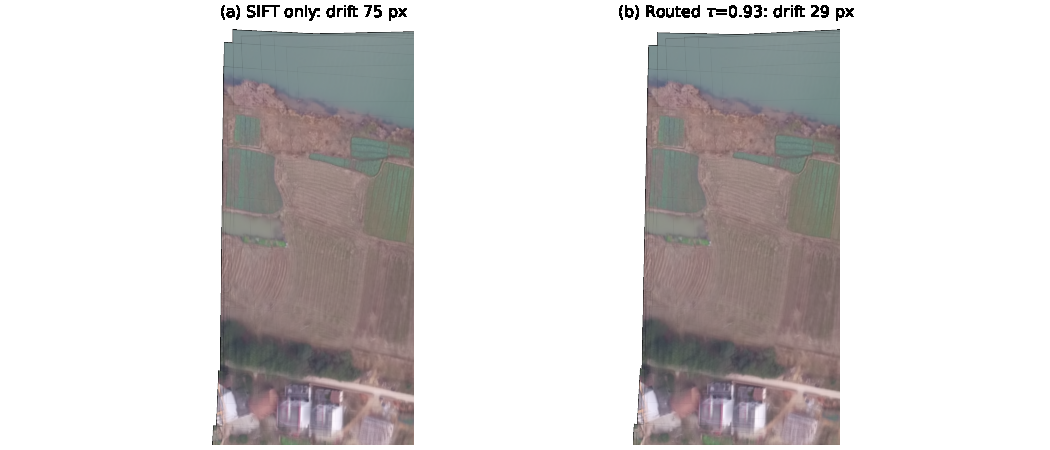
\includegraphics[width=\columnwidth]{figures/fig_mosaic_village.pdf}
\caption{Ảnh mosaic dựng lại của cửa sổ \texttt{village} (46 frame): (a) Baseline cổ điển
(chỉ SIFT tuần tự), (b) Phân luồng đề xuất ($\tau_{\mathrm{ncc}}{=}0{,}93$). Đường viền ngoài
là biên frame đã warp; sai số drift tích luỹ cuối giảm từ 75,3\,px xuống còn 28,5\,px.}
\label{fig:mosaic_village}
\end{figure}

\begin{figure}[t]
\centering
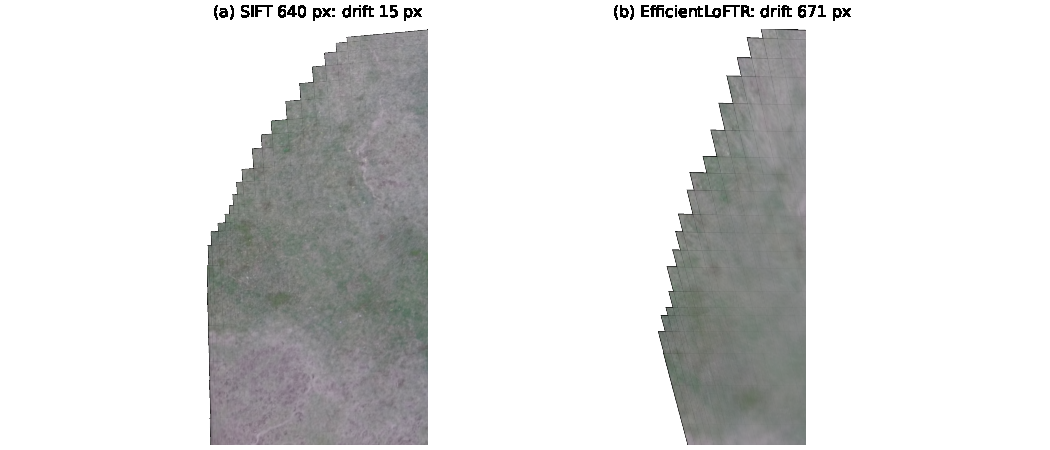
\includegraphics[width=\columnwidth]{figures/fig_mosaic_grass.pdf}
\caption{Cùng 46 frame của \texttt{grass} không phục hồi: (a) Baseline cổ điển
(SIFT 640\,px), (b) Baseline học sâu (Efficient LoFTR). Răng cưa bên phải là lỗi hình học tích
luỹ 671,3\,px so với chuỗi tham chiếu trên vùng nông nghiệp đồng nhất.}
\label{fig:mosaic_grass}
\end{figure}

\begin{figure}[t]
\centering
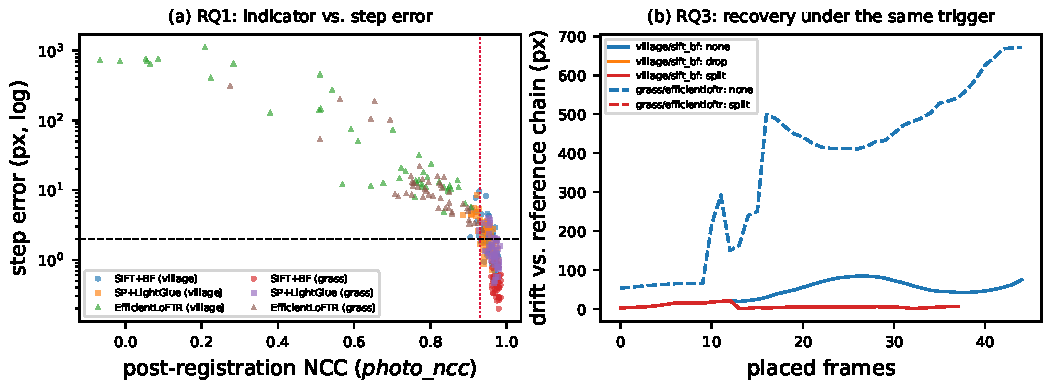
\includegraphics[width=\columnwidth]{figures/fig_rq1_rq3.pdf}
\caption{(a) Sai số bước theo chỉ báo NCC sau ghép trên cả hai cửa sổ và ba
matcher; đường gạch ngang = ranh giới 2\,px, đường chấm = ngưỡng được chọn.
(b) Drift so với chuỗi tham chiếu của các chiến lược RQ3 dưới cùng ngưỡng.
Tách mảnh đặt lại hệ toạ độ ở mỗi mảnh, nên đường của nó là từng đoạn, không
phải một chuỗi liền.}
\label{fig:rq1rq3}
\end{figure}

\begin{figure}[t]
\centering
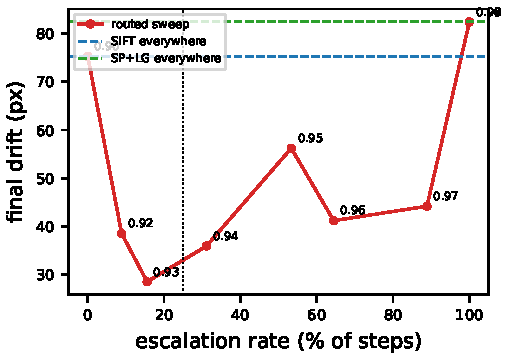
\includegraphics[width=\columnwidth]{figures/fig_tau.pdf}
\caption{Đánh giá RQ2 trên \texttt{village}: (a) Đường cong trôi dạt tích luỹ qua các frame
so sánh hai baseline cố định (chỉ SIFT và chỉ SP+LG) với bộ phân luồng hai tầng đề xuất
($\tau_{\mathrm{ncc}}{=}0{,}93$). (b) Quét ngưỡng tỉ lệ leo thang so với drift cuối dưới ngân
sách 25\%. Drift không đơn điệu theo $\tau$, chứng minh việc leo thang mù làm suy biến hình học toàn cục.}
\label{fig:tau}
\end{figure}

\subsection{RQ3: phục hồi dưới cùng một ngưỡng}
Bảng~\ref{tab:rq3} báo cáo cả hai cửa sổ. Trên village (7 trigger ban đầu),
\emph{tách mảnh} đặt đủ 46 frame thành 8 mảnh con, nối được 38 trên 45 bước với
drift nội bộ lớn nhất 21,7\,px; \emph{bỏ frame} và \emph{neo} chỉ giữ 14/46
frame (13 bước nối được, cùng mức trần 21,7\,px), vì bỏ một frame làm tăng
khoảng trống chồng lấn của cặp kế tiếp và ngưỡng lại kích hoạt (7 trigger ban
đầu nở thành 32). \emph{neo} cho kết quả y hệt \emph{bỏ frame} ở đây: khi mọi
ứng viên còn lại đều đã bị loại hoặc chưa được đặt, không có frame neo nào an
toàn. Hình~\ref{fig:mosaic_split} cho thấy chiến lược tách mảnh thực sự tạo ra
cái gì.

Trên grass với Efficient LoFTR, 44 trong 45 bước bị gắn cờ. \emph{bỏ frame} và
\emph{neo} đặt được đúng một frame (bản đồ không tồn tại); \emph{tách mảnh} giữ
đủ 46 frame nhưng suy biến thành 45 mảnh một frame với đúng một bước nối được.
Drift thấp ở đó là hệ quả của việc chặt vụn, không phải bằng chứng của một bản
đồ được cứu.

\begin{figure}[t]
\centering
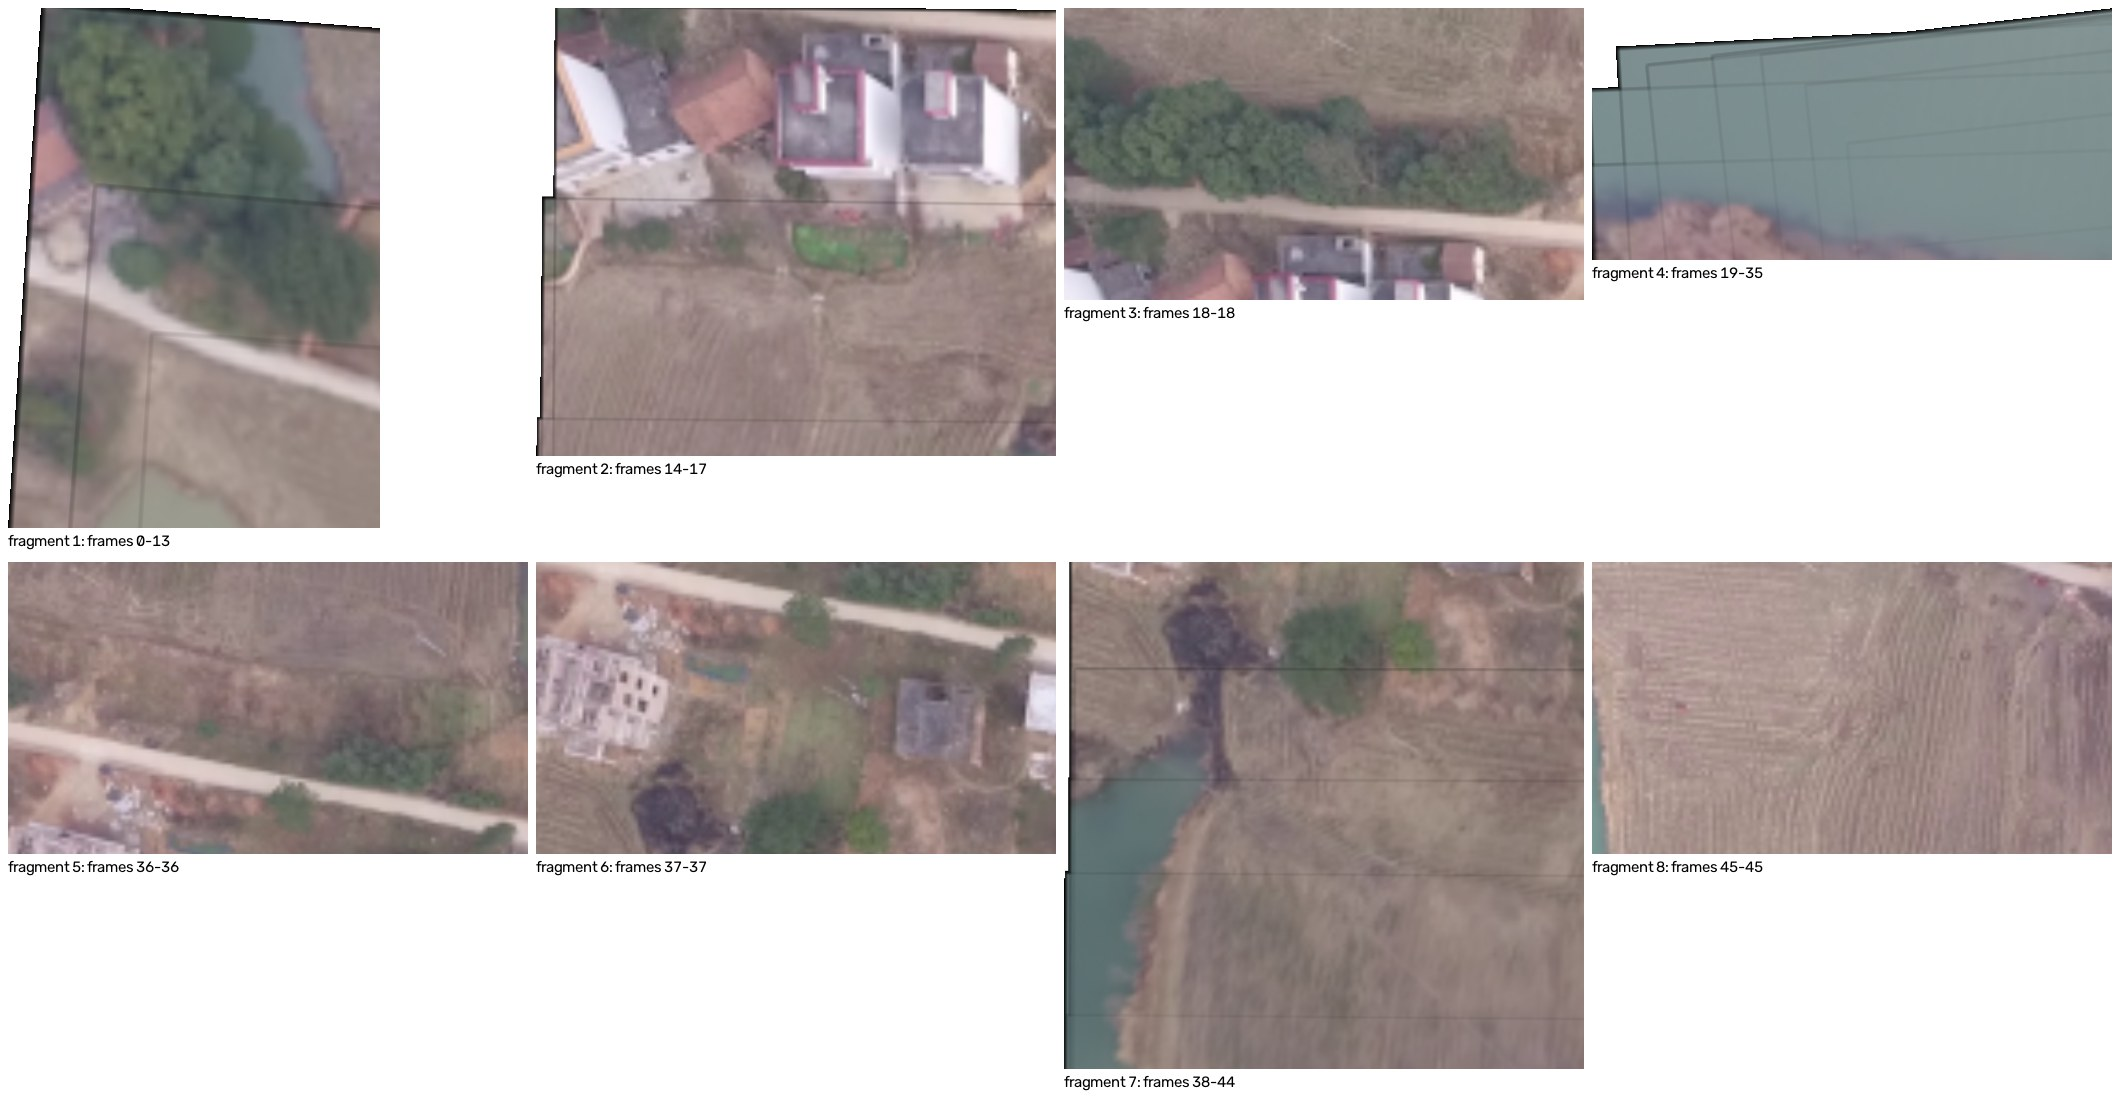
\includegraphics[width=\columnwidth]{figures/mosaic_village_split.jpg}
\caption{Chiến lược tách mảnh trên \texttt{village}: vẫn 46 frame đó, cắt tại 7
bước bị gắn cờ thành 8 mảnh, mỗi mảnh một hệ toạ độ riêng. Frame không mất,
nhưng đầu ra là 8 mặt phẳng rời rạc, trong đó bốn mảnh (3, 5, 6 và 8) chỉ có
một frame.}
\label{fig:mosaic_split}
\end{figure}

\begin{table}[t]
\caption{RQ3: các chiến lược phục hồi ở ngưỡng mà RQ2 đã chọn (village
$\tau{=}0{,}93$, grass $\tau{=}0{,}96$). Drift là mức lớn nhất trong nội bộ một
chuỗi; tách mảnh đặt lại hệ toạ độ cho từng mảnh, và n/a nghĩa là không đặt
được frame nào nên không có gì để đo.}\label{tab:rq3}
\centering\footnotesize
\setlength{\tabcolsep}{3pt}
\begin{tabular}{llccr}
\toprule
Cửa sổ / matcher & Chiến lược & Frame giữ & Mảnh con & Drift (px) \\
\midrule
village / SIFT & không cứu & 46/46 & 1  & 84,6 \\
village / SIFT & bỏ frame  & 14/46 & 1  & 21,7 \\
village / SIFT & neo       & 14/46 & 1  & 21,7 \\
village / SIFT & tách mảnh & 46/46 & 8  & 21,7 \\
grass / ELoFTR & không cứu & 46/46 & 1  & 671,3 \\
grass / ELoFTR & bỏ frame  & 1/46  & 1  & n/a \\
grass / ELoFTR & tách mảnh & 46/46 & 45 & 2,7 \\
\bottomrule
\end{tabular}
\end{table}

\section{Thảo luận}\label{sec:disc}
\textbf{Rẻ không có nghĩa là có ích.} Số điểm khớp và số inlier, những chỉ
báo mà hầu hết luật nhận/loại dùng, không mang tín hiệu dùng được ở cấp bước
trong cửa sổ của chúng tôi, và dữ liệu còn đảo ngược chiều đã khai báo (càng ít
điểm khớp càng bị coi là đáng ngờ):
matcher sinh nhiều điểm khớp vẫn có thể đặt chúng nhất quán với một hình học
sai. Các chỉ báo tính \emph{sau} khi đăng ký (tương phản quang học, sai số nội
tại, độ chồng lấn sau chiếu) mới mang tín hiệu. Hệ quả thực tế: chúng không thể
đánh giá trước khi matching, nên ngưỡng của chúng tôi là một cổng hậu kiểm trên
kết quả của matcher rẻ, không phải bộ dự báo trước matching.

\textbf{Tiêu nhiều tính toán hơn không đơn điệu theo chất lượng.}
Luôn-học-sâu kết thúc tệ hơn chỉ-SIFT trên village, và việc leo thang ở ảnh gốc
cải thiện sai số từng bước nhưng không chuyển thành drift chuỗi thấp hơn. Cơ
chế khả dĩ: bản đồ tích luỹ là sản phẩm của cả chuỗi, không phải của sai số
trung bình từng bước; một $H_i$ ``tốt hơn'' cục bộ làm thay đổi hình học mà các
frame sau phải bù lại. Chúng tôi coi đây là giả thuyết; muốn kiểm thì phải thay
đổi tập bước leo thang độc lập với ngưỡng.

\textbf{Chọn ngưỡng mới là phần khó.} Hình~\ref{fig:tau} cho thấy đường quét có
dạng chữ U: 15,6\% leo thang là điểm tốt nhất đo được, còn leo thang một nửa số
bước (53\%) lại tệ hơn cả không leo thang bước nào. Luật ngân sách (``$\tau$
lớn nhất sao cho tỉ lệ leo thang dưới 25\%'') cho 0,93/0,96 trên hai cửa sổ,
nhưng một luật giả định tính đơn điệu trên một khoảng mà thước đo không đơn
điệu thì chỉ đúng trong phạm vi những cửa sổ đã dùng để khớp nó.

\textbf{Đánh đổi của phục hồi là frame so với tính liên thông.} Tách mảnh bảo
toàn số frame nhưng làm vụn bản đồ (8 mảnh cho 46 frame, 45 mảnh trong ca suy
biến); bỏ frame/neo giữ được tính liên tục của phần sống sót nhưng bị dây
chuyền dưới một ngưỡng bảo thủ, mất 70\% số frame ở đây. Bên nào tốt hơn phụ
thuộc vào việc dùng bước sau cần độ phủ hay cần một mặt phẳng hình học duy
nhất, câu hỏi mà số liệu của chúng tôi chưa trả lời được, và đó là lý do nên
xem ảnh ghép của từng chiến lược trước khi kết luận.

\section{Giới hạn}
\textbf{Thước đo sai số.} Mọi sai số là bất đồng với chuỗi tham chiếu SIFT ảnh
gốc, và chính chuỗi đó cũng tích luỹ sai số; chưa có phần nào được kiểm chứng
với hình học thực địa (chưa đối chiếu GCP/ảnh trực giao trong bản nháp này),
nên không được đọc các giá trị drift tuyệt đối như độ chính xác định vị.

\textbf{Mẫu.} Hai trong 14 gói công khai của NPU Drone-Map, hai cửa sổ được
chọn \emph{vì} chúng khó. Tỉ lệ bước sai (21/45, 6/38, 45/45) là đặc tính của
cách chọn đó, không phải kỳ vọng khi triển khai. Chưa có sequence giữ riêng, và
ngưỡng lẫn ngân sách chưa được thử lại trên các gói còn lại.

\textbf{Chọn mẫu và đa giả thuyết.} Chỉ báo, chiều, mốc 2\,px và $\tau$ đều
được chọn khi đã nhìn vào chính các cửa sổ này; chiều được cố định trước để loại
lỗ hổng rõ nhất, nhưng kết quả vẫn là khám phá chứ chưa phải xác nhận. 45 bước
cũng phụ thuộc thời gian, không phải 45 quan sát độc lập.

\textbf{Kế toán chi phí.} Cột thời gian chỉ đo tầng matcher. RANSAC, warp, các
phép kiểm quang học và quyết định rủi ro đều không tính, nên bản nháp này không
ủng hộ bất kỳ tuyên bố nào về độ trễ end-to-end; chi phí phân luồng thực tế cao
hơn 13,3\,s và chi phí của luôn-học-sâu cũng còn phần hậu xử lý chưa tính.

\textbf{Tích hợp.} RQ3 chạy một matcher cố định cho mỗi cửa sổ và không dùng
các tuyến phân luồng từ RQ2; một lần chạy end-to-end ``rẻ $\to$ leo thang $\to$
phục hồi'', ảnh ghép của nó, và thước đo liên thông giữa các mảnh vẫn còn
thiếu. Toàn bộ thời gian đo trên một máy chỉ có CPU.

\section{Kết luận}
Trên một pipeline homography tích luỹ cho video UAV, các chỉ báo rẻ dự báo được
rủi ro cấp bước không phải là số điểm khớp mà các luật nhận/loại thường dùng,
mà là bằng chứng sau khi ghép; một bộ phân luồng cổ-điển-trước với ngưỡng chọn
theo ngân sách đã giảm drift cuối 62\% với chi phí gấp 4,1 lần matcher rẻ, trong
khi gọi matcher học sâu cho mọi bước thì vừa chậm vừa tệ hơn; và dưới cùng một
ngưỡng, tách mảnh giữ được toàn bộ frame trong khi bỏ frame/neo bị dây chuyền
xuống còn 14/46. Các bước tiếp theo, theo thứ tự: chạy lại nguyên notebook trên
các gói giữ riêng, nối phân luồng với phục hồi thành một lần chạy end-to-end có
đo thời gian toàn pipeline, kiểm chứng với hình học thực địa, và xem ảnh ghép
của từng chiến lược.

\begin{thebibliography}{00}
\bibitem{lowe2004} D. G. Lowe, ``Distinctive image features from scale-invariant keypoints,'' \emph{Int. J. Comput. Vis.}, vol. 60, no. 2, pp. 91--110, Nov. 2004, doi: 10.1023/B:VISI.0000029664.99615.94.
\bibitem{rublee2011} E. Rublee, V. Rabaud, K. Konolige, and G. Bradski, ``ORB: An efficient alternative to SIFT or SURF,'' in \emph{Proc. IEEE Int. Conf. Comput. Vis. (ICCV)}, Barcelona, Spain, 2011, pp. 2564--2571, doi: 10.1109/ICCV.2011.6126544.
\bibitem{fischler1981} M. A. Fischler and R. C. Bolles, ``Random sample consensus: A paradigm for model fitting with applications to image analysis and automated cartography,'' \emph{Commun. ACM}, vol. 24, no. 6, pp. 381--395, Jun. 1981, doi: 10.1145/358669.358692.
\bibitem{detone2018} D. DeTone, T. Malisiewicz, and A. Rabinovich, ``SuperPoint: Self-supervised interest point detection and description,'' in \emph{Proc. IEEE/CVF Conf. Comput. Vis. Pattern Recognit. Workshops (CVPRW)}, Salt Lake City, UT, USA, 2018, pp. 224--236, doi: 10.1109/CVPRW.2018.00060.
\bibitem{lindenberger2023} P. Lindenberger, P.-E. Sarlin, and M. Pollefeys, ``LightGlue: Local feature matching at light speed,'' in \emph{Proc. IEEE/CVF Int. Conf. Comput. Vis. (ICCV)}, Paris, France, 2023, pp. 8845--8855, doi: 10.1109/ICCV51070.2023.00812.
\bibitem{sun2021} J. Sun, Z. Shen, Y. Wang, H. Bao, and X. Zhou, ``LoFTR: Detector-free local feature matching with transformers,'' in \emph{Proc. IEEE/CVF Conf. Comput. Vis. Pattern Recognit. (CVPR)}, Nashville, TN, USA, 2021, pp. 8922--8931, doi: 10.1109/CVPR46437.2021.00881.
\bibitem{wang2024} Q. Wang, J. Zhang, K. Han, X. Peng, and C. Shen, ``Efficient LoFTR: Semi-dense local feature matching with sparse-like speed,'' in \emph{Proc. IEEE/CVF Conf. Comput. Vis. Pattern Recognit. (CVPR)}, Seattle, WA, USA, 2024, pp. 21544--21554, doi: 10.1109/CVPR52733.2024.02035.
\bibitem{potlapalli2024} P. Potlapalli, P. Lindenberger, and M. Pollefeys, ``XFeat: Accelerated features for lightweight image matching,'' in \emph{Proc. IEEE/CVF Conf. Comput. Vis. Pattern Recognit. (CVPR)}, Seattle, WA, USA, 2024, pp. 19163--19172, doi: 10.1109/CVPR52733.2024.01811.
\bibitem{hwang2026} D. Hwang, S. Lee, and J. Park, ``Real-time 2D orthomosaic mapping using CPU-based incremental homography matrix estimation with UAV video,'' \emph{Appl. Sci.}, vol. 16, no. 4, Art. no. 2133, Feb. 2026, doi: 10.3390/app16042133.
\bibitem{li2023} X. Li, Y. Liu, C. Wang, and Z. Zhang, ``A real-time incremental video mosaic framework for UAV remote sensing,'' \emph{Remote Sens.}, vol. 15, no. 8, Art. no. 2127, Apr. 2023, doi: 10.3390/rs15082127.
\bibitem{dronezaic} M. Kharismawati and D. Kazic, ``DroneZaic: A robust end-to-end pipeline for mosaicking freely flown aerial video of agricultural fields,'' \emph{Plant Phenome J.}, vol. 8, no. 1, Art. no. e70033, Feb. 2025, doi: 10.1002/ppj2.70033.
\bibitem{chen2022} J. Chen, J. Yang, C. Deng, and H. Shen, ``UAV video stitching based on optimal seamline and half-projective warp,'' \emph{Remote Sens.}, vol. 14, no. 5, Art. no. 1068, Mar. 2022, doi: 10.3390/rs14051068.
\bibitem{kim2025} J. Kim and S. Kim, ``Robust UAV image mosaicking using SIFT and LightGlue,'' \emph{Int. Arch. Photogramm. Remote Sens. Spatial Inf. Sci.}, vol. XLVIII-2/W11-2025, pp. 169--173, 2025, doi: 10.5194/isprs-archives-XLVIII-2-W11-2025-169-2025.
\bibitem{gaisbauer2025} S. Gaisbauer, P. Gyawali, Q. Zhang, O. Wysocki, and B. Jutzi, ``To glue or not to glue? Classical vs learned image matching for mobile mapping cameras to textured semantic 3D building models,'' \emph{ISPRS Ann. Photogramm. Remote Sens. Spatial Inf. Sci.}, vol. X-1/W2-2025, pp. 69--76, 2025, doi: 10.5194/isprs-annals-X-1-W2-2025-69-2025.
\bibitem{zaffar2024} M. Zaffar, L. S. F. Ribeiro, S. Ehsan, and M. Milford, ``On the estimation of image-matching uncertainty in visual place recognition,'' in \emph{Proc. IEEE/CVF Conf. Comput. Vis. Pattern Recognit. (CVPR)}, Seattle, WA, USA, 2024, pp. 17751--17761, doi: 10.1109/CVPR52733.2024.01680.
\bibitem{sferrazza2024} C. Sferrazza, Y. Chen, S. Shen, and P. Abbeel, ``To match or not to match: Evaluating keypoint matching confidence for visual place recognition,'' in \emph{Proc. IEEE/CVF Conf. Comput. Vis. Pattern Recognit. Workshops (CVPRW)}, Seattle, WA, USA, 2024, pp. 2883--2892, doi: 10.1109/CVPRW63382.2024.00293.
\bibitem{barath2023} D. Barath, L. Cavalli, and M. Pollefeys, ``A large-scale homography benchmark,'' in \emph{Proc. IEEE/CVF Conf. Comput. Vis. Pattern Recognit. (CVPR)}, Vancouver, BC, Canada, 2023, pp. 17679--17688, doi: 10.1109/CVPR52729.2023.01695.
\bibitem{yuan2024} H. Yuan, D. Peng, and M. Dong, ``Comparative analysis of color space transformations on feature-based image registration,'' \emph{J. Imaging}, vol. 10, no. 5, Art. no. 105, May 2024, doi: 10.3390/jimaging10050105.
\bibitem{ivashechkin2021} M. Ivashechkin, D. Barath, and J. Matas, ``VSAC: Efficient and accurate estimator for H and F,'' in \emph{Proc. IEEE/CVF Int. Conf. Comput. Vis. (ICCV)}, Montreal, QC, Canada, 2021, pp. 6003--6012, doi: 10.1109/ICCV48922.2021.00595.
\bibitem{uasthn} J. Xiao and G. Loianno, ``UASTHN: Uncertainty-aware deep homography estimation for UAV satellite--thermal geo-localization,'' arXiv preprint arXiv:2502.01035, 2025.
\bibitem{dalglue} H. Zhang, H. He, Y. Zhou, and F. Lei, ``Efficient image matching for UAV visual navigation via DALGlue,'' \emph{Sci. Rep.}, vol. 15, Art. no. 37684, 2025, doi: 10.1038/s41598-025-37684-2.
\bibitem{map2dfusion} S. Bu, Y. Zhao, G. Wan, and Z. Liu, ``Map2DFusion: Real-time incremental UAV image mosaicing based on monocular SLAM,'' in \emph{Proc. IEEE/RSJ Int. Conf. Intell. Robots Syst. (IROS)}, Daejeon, South Korea, 2016, pp. 4564--4571, doi: 10.1109/IROS.2016.7759672.
\end{thebibliography}

\end{document}
